\section{Implementation and tests}

Before experimenting the real robots in the environment, it is necessary to develop and test the solutions on a simulator. To this end, we report here the development of a simulated environment for the project and some preliminary results.


\subsection{Simulator environment}

The simulation environment is based on 2D Stage simulator, that is integrated in the ROS infrastructure. The choice of a 2D simulator (instead of a 3D one) is motivated by: 1) the need of modeling and testing high-level behaviors of the robot that does not involve 3D perception, 2) the possibility of using the simulator for multiple robots and other moving elements representing people in the environment, 3) the possibility of using the simulator on standard laptop, thus not requiring advanced graphical cards for running 3D simulations.

\begin{figure}
\centering
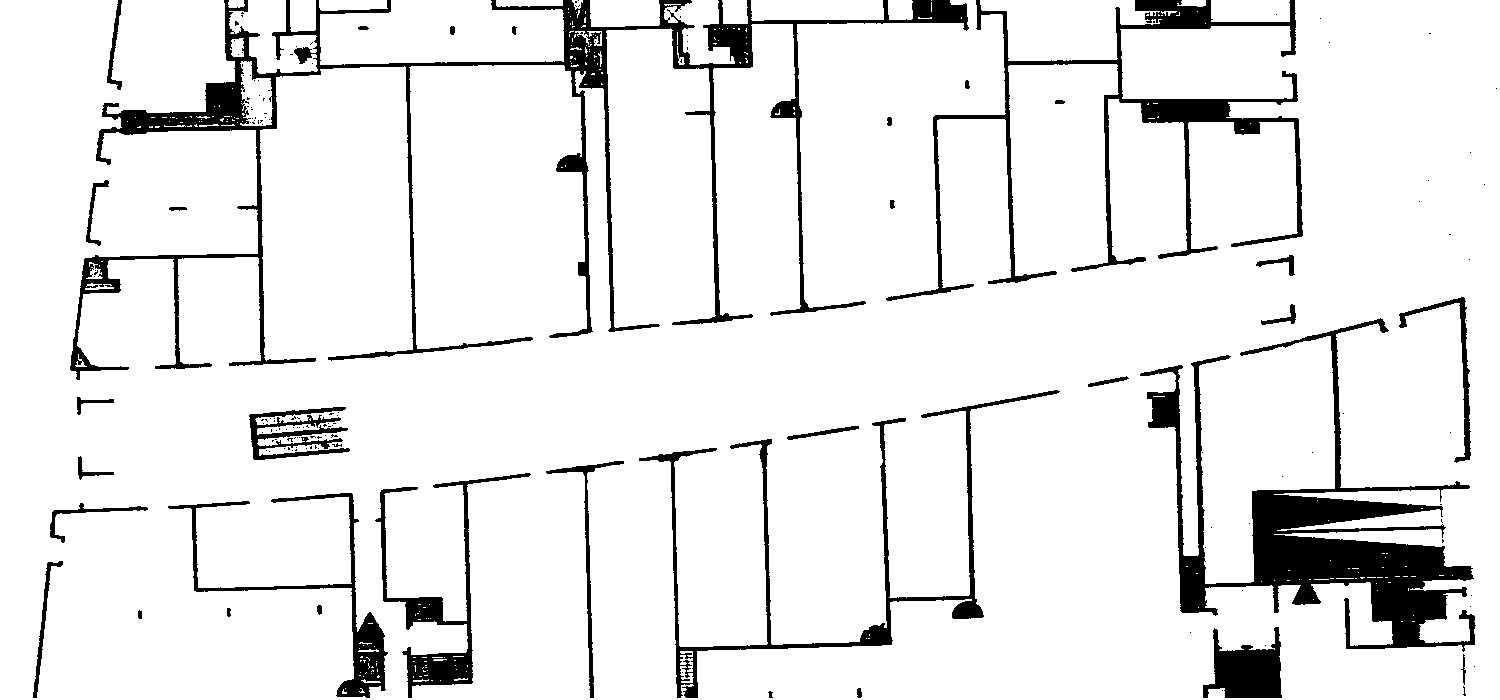
\includegraphics[width=0.95\textwidth]{fig/Rive1.png}
\caption{2D map of the \emph{Rive de l'orne} shopping center.}
\label{fig:stage}
\end{figure}


In the Stage simulator the following map of the \emph{Rive de l'orne} shopping center has been realized. In Figure \ref{fig:stage} a section of the shopping mall in which we will deploy the prototypes is shown.
Additional maps have been realized for reproducing the environments of the partners in which some experiments will be performed.

The Stage environment models one or more robots that have the same 2D sensor and actuator configurations as the real ones and some additional mobile obstacles that represent people moving in the environment. Several behaviors can be tested in this simulated environment such as: 2D perception of human behaviors, human-robot social navigation (e.g., following a person or guiding a person), safe navigation in the environment.

The Stage environment has been fully realized and tested and this configuration will be used as a reference also for the development of the real robotic system.

\subsection{Plan generation and execution tests}

The following tests have been performed in the simulator to verify the suitability of the proposed software architecture and of its components. In particular, we have used the simulated environment to assess the suitability of the AI components described in the previous section.

\begin{itemize}
\item Simple Move-To behavior: moving the robot from one place to another allows for testing the map description, path planning, and the global architecture.
\item Patrol behavior: moving the robot across several places allows for testing the sequential decision-making, along with the dynamic addition of new places to visit or new obstacles.
\item Simple interaction: going to some people for initiating an interaction allows for testing the difficulties introduced by non-stationary goals, along with the dialog system. It also makes it easier to test for branching behaviors since the dialogs may have several different outcomes.
\end{itemize}

When executing these behaviors, we have tested many possible causes of failures (that are implemented in Stage by manually moving with the mouse elements that represents people in the environment or by injecting specific conditions through a GUI). We have thus verified that the system is able to respond quickly and effectively also to unpredicted and non-modeled events.

At this moment, we do not aim at a quantitative evaluation of the developed components, but at demonstrating the entire flow of information and the feasibility of the approach.
The results of the tests confirm that the effectiveness of the adopted solution integrating the three main components described in this paper: KB representation and reasoning, MDP planner and PNP execution. Moreover, we have successfully experimented in several cases how the feedback provided by the execution layer can be used to improve the model and thus the robustness of the plan generated by the planner.


